\chapter{Usage information}

The \OFEname \ application is available on Linux, Windows and MacOSX platforms.
We encourage you to use \OFEname \ program on Linux platform as it is the development and usually used platform. The following instructions mainly applies to Linux platforms.   

\section{Installation}

On linux platforms, the \OFEname \ software is available as distribution packages (deb, rpm) or archive files (tar.gz, tar.bz2).  
The recommanded way to install is to use packages for your Linux distribution. If you want to use archive files, you have to unarchive the software according to the directory tree.\\
Once installed, the \texttt{openfluid-engine} command should be available. You can check it by running the command \texttt{openfluid-engine} \verb?--?\texttt{help} or \texttt{openfluid-engine} \verb?--?\texttt{version} in your favorite terminal. You are now ready to run your first simulation.  

\section{Input dataset}

Before running the simulation, the input dataset must be built.
An \OFEname \ input dataset includes different informations, shared into many files:
\begin{itemize}
  \item the spatial domain definition
  \item the flux model definition
  \item the spatial domain input data 
  \item the discrete events
  \item the run configuration
  \item the outputs configuration
\end{itemize}

\noindent All these files must be placed into any directory that can be reached by the
engine. The default searched directory is a directory named
\texttt{.openfluid/engine/OPENFLUID.IN} and located into the user home
directory (the user home directory may vary, depending on the used operating
system). If you prefer to place your dataset in another directory, you can
specify it using command line options passed to the engine (\texttt{-i} or \verb?--?\texttt{input-dir}).\\

\noindent In order to build these files, we encouraged you to use a good text editor, or better, an XML editor.
You can also use custom scripts or macros in specialized sotware, such as spreadsheets or Geographic Information Systems (GIS), to generate automatically the input dataset.

\bigskip

\section{Engine sequence}

\textbf{TODO}


\bigskip


\section{Run the simulation}

To run the simulation, if the dataset is located in the default searched directory, simply run the command \texttt{openfluid-engine} in your favorite terminal. 
To specify a different input dataset directory, use the \texttt{-i} or \verb?--?\texttt{input-dir} command line option.    

\bigskip

\begin{latexonly}
\begin{center}
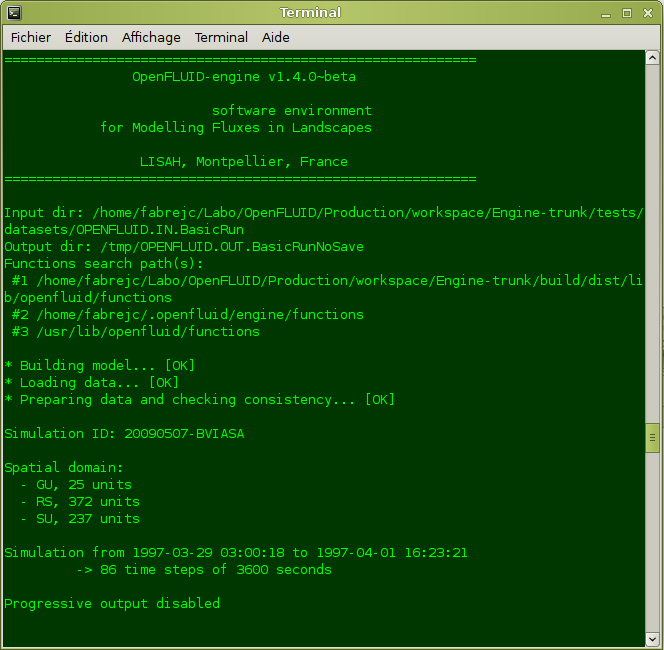
\includegraphics[scale=0.6]{common/graphics/oferun.png}
\end{center}
\end{latexonly}

\begin{htmlonly}
\begin{center}
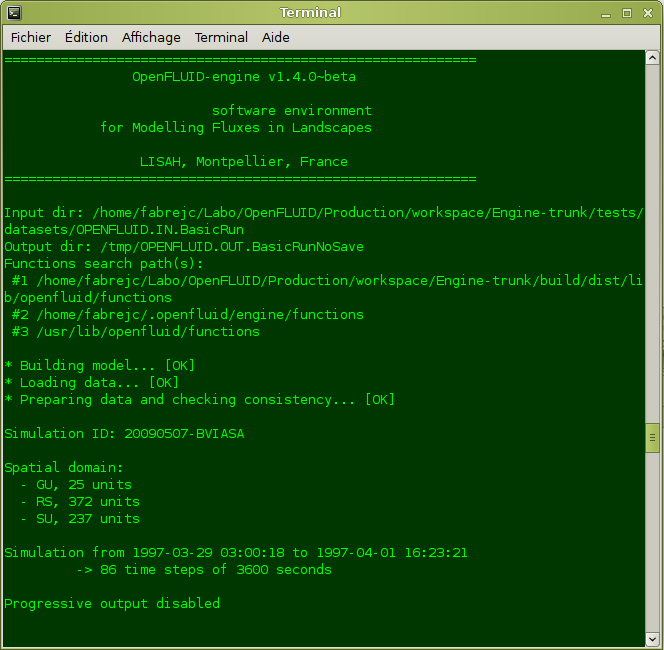
\includegraphics[scale=1]{common/graphics/oferun.png}
\end{center}
\end{htmlonly}

\section{Explore the results}

The results are stored in files, gathered by spatial unit. In each files, the values for variables are stored as columns, each row corresponfing to a data exchange time step (represented as a date and time).
The format of the files depends on the configuration of outputs, set through the \texttt{run.xml} file.
The default output directory is a directory named \texttt{.openfluid/engine/OPENFLUID.OUT} and located into the user home directory (the user home directory may vary, depending on the used operating system).
If you prefer to save your outputs in another directory, you can specify it using command line options passed to the engine (\texttt{-o} or \verb?--?\texttt{output-dir}).\\

\noindent In order to process the results of your simulations, we encourage you to use software environments such as R, Scilab or Octave, spreadsheets such as OpenOffice Calc, GIS such as GRASS or QGIS.   
